\documentclass[a4paper,oneside,12pt]{report}

\usepackage{styles/tez}





% COVER PAGE
\title{TEZ BAŞLIĞI}
\setIngilizceBaslik{THESIS TITLE}



% BEGIN OF DOCS
\begin{document}
\pagenumbering{roman}
\newpage
\thispagestyle{empty}
\singlespacing
\vspace*{3cm}
Kapak sayfasıdır. Word dosyasında hazırlanması tavsiye edilir.

\newpage
\thispagestyle{empty}
\singlespacing
\vspace*{3cm}
Kapak sayfasından sonra gelen boş sayfadır. Buradaki metnin silinmesi gerekir. Diğer kısımlar silinmemelidir. 

Onay sayfası jüri adedine göre ve eş danışman durumuna göre düzenlenmelidir. Düzenlenirken sadece yazı kısımları silinmeli tablo ayarları değiştirilmemelidir. Onay sayfasının da Word'de hazırlanıp pdf olarak çıktısı alındıktan sonra bastırılması daha uygun olacaktır.

\newpage
\paragraph{}
\singlespacing
\vspace*{2cm}
\noindent
BTÜ, Lisansüstü Eğitim Enstitüsü’nün 22102312 numaralı Yüksek Lisans/Doktora öğrencisi, Adem ADEMOĞLU, ilgili yönetmeliklerin belirlediği gerekli tüm şartları yerine getirdikten sonra hazırladığı “TEZ BAŞLIĞI” başlıklı tezini, aşağıda imzaları olan jüri üyeleri önünde başarı ile sunmuştur.

\vspace{2cm}
\begin{tabular}{p{4cm} p{6cm} p{3.5cm}}  
\textbf{Tez Danışmanı:} & \textbf{Ünvan Adı SOYADI} & \dotfill \\  
& Bursa Teknik Üniversitesi  & \\
\end{tabular}

\vspace{0.6cm}
\begin{tabular}{p{4cm} p{6cm} p{3.5cm}}  
	\textbf{İkinci Danışman:} & \textbf{Ünvan Adı SOYADI} & \dotfill \\  
	(Varsa) & Kurum   & \\
\end{tabular}

\vspace{0.6cm}
\begin{tabular}{p{4cm} p{6cm} p{3.5cm}}  
	\textbf{Jüri Üyeleri:} & \textbf{Ünvan Adı SOYADI} & \dotfill \\
	& Kurum   & \\
\end{tabular}

\vspace{0.6cm}
\begin{tabular}{p{4cm} p{6cm} p{3.5cm}}  
	 & \textbf{Ünvan Adı SOYADI} & \dotfill \\
	 & Kurum   & \\
\end{tabular}

\vspace{0.6cm}
\begin{tabular}{p{4cm} p{6cm} p{3.5cm}}  
	(Varsa)& \textbf{Ünvan Adı SOYADI} & \dotfill \\
	& Kurum   & \\
\end{tabular}

\vspace{0.6cm}
\begin{tabular}{p{4cm} p{6cm} p{3.5cm}}  
	(Varsa)& \textbf{Ünvan Adı SOYADI} & \dotfill \\
	& Kurum   & \\
\end{tabular}

\vspace{2cm}
\begin{tabular}{p{4cm} p{5.5cm}}  
	\textbf{Teslim Tarihi} & \textbf{: 02.02.2025} \\
	\textbf{Savunma Tarihi} & \textbf{: 02.02.2025} \\
\end{tabular}

\clearpage
\paragraph{}
\vfill
20.04.2016 tarihli Resmi Gazete’de yayımlanan Lisansüstü Eğitim ve Öğretim Yönetmeliğinin 9/2 ve 22/2 maddeleri gereğince; Bu Lisansüstü teze, Bursa Teknik Üniversitesi’nin abonesi olduğu intihal yazılım programı kullanılarak Lisansüstü Eğitim Enstitüsü’nün belirlemiş olduğu ölçütlere uygun rapor alınmıştır.

Bu tez, Bursa Teknik Üniversitesi Bilimsel Araştırma Projeleri Koordinatörlüğünün ........ numaralı projesi ile desteklenmiştir.

Bu tez, ....... numaralı ..................... projesi ile desteklenmiştir.

\clearpage
\paragraph{}
\vskip 36 pt
\begin{center}
	\textbf{İNTİHAL BEYANI}
\end{center}
Bu tezde görsel, işitsel ve yazılı biçimde sunulan tüm bilgi ve sonuçların akademik ve etik kurallara uyularak tarafımdan elde edildiğini, tez içinde yer alan ancak bu çalışmaya özgü olmayan tüm sonuç ve bilgileri tezde kaynak göstererek belgelediğimi, aksinin ortaya çıkması durumunda her türlü yasal sonucu kabul ettiğimi beyan ederim.
\begin{flushright}
	\begin{tabular}{l r r}
		&Öğrencinin Adı Soyadı:& Ahmet Ahmetoğlu \\
		&&\\
		&İmzası:& \\
	\end{tabular}
\end{flushright}

\clearpage

\begin{flushright}
	\vspace*{\fill}
	\textbf{\textit{Aileme,}} % Italicized dedication
	\vspace*{\fill}
\end{flushright}

% ACK PAGE
\begin{acknowledgements}
Önsöz bölümünün içerisindeki metinler 1 satır aralıklı yazılır. Tezin ilk sayfası
niteliğinde yazılan önsöz iki sayfayı geçmez.

Tezi destekleyen kurumlara ve yardımcı olan kişilere bu kısımda teşekkür edilir.
Önsöz metninin altında sağa dayalı olarak ad-soyad, sola dayalı olarak ay, yıl
biçiminde tarih yazılır. Bu iki unsur aynı hizada olur.
\vskip 36pt

\begin{minipage}{0.5\textwidth}
	\raggedright
	Şubat 2025
\end{minipage}%
\begin{minipage}{0.5\textwidth}
	\raggedleft
	Ahmet AHMEDOĞLU \\[2pt]
	{(Meslek)}
\end{minipage}

\end{acknowledgements}

% CONTENTS AND LIST OF FIG AND TABLE PAGES
\tableofcontents

% LIST OF ABBREV PAGE
\begin{abbreviations}
	% Abbreviations in alphabetical order
	\sym{AIC}{Akaike Information Criteria}
	\sym{ANN}{Artificial Neural Network}
	\sym{App}{Appendix}
	\sym{BP}{Backpropagation}
	\sym{CGI}{Common Gateway Interface}
	\sym{ESS}{Error sum-of-squares}
	\sym{GARCH}{Generalized Autoregressive Conditional Heteroskedasticity}
	\sym{GIS}{Geographic Information Systems}
	\sym{HCA}{Hierarchical Cluster Analysis}
	\sym{Mbps}{Megabits per second}
	\sym{St}{Station}
	\sym{SWAT}{Soil and Water Assessment Tool}
\end{abbreviations}

% LIST OF SYMBOLS PAGE
\begin{symbols}
	% The title will be typeset as "LIST OF SYMBOLS".
	% Use a separate \sym command for each symbols definition.
	% First, Latin symbols in alphabetical order
	\sym{$\alpha$}{Asal gerilme doğrultusundan sapma açısı}
	\sym{$\rho$}{Yoğunluk}
	\sym{$\sigma_x,\sigma_y,\sigma_{x,y}$}{Kabuk iç gerilmeleri}
	\sym{C}{Dokunun kapasitansı}
	\sym{$\mathbf{H}$}{Isı miktarı}
	\sym{$\mathbf{M_x,M_y,M_{xy}}$}{Moment Bileşenleri}
	\sym{$\mathbf{N_x,N_y,N_{xy}}$}{Normal Kuvvet Bileşenleri}
	\sym{$\mathbf{q}$}{Faz yükü}
	\sym{$\mathbf{XC}$}{Kapasitif reaktans}
\end{symbols}

\listoftables
\listoffigures

% OZET PAGE
\begin{ozet}
Özet hazırlanırken 1 satır boşluk bırakılır.
Türkçe tezlerde, Türkçe ve İngilizce özet 300 ile 750 kelime arasında olmalıdır.
İngilizce tezlerde ise, İngilizce ve Türkçe özet 300 ile 750 kelime arasında olmalıdır.
Özetlerde tezde ele alınan konu kısaca tanıtılarak, kullanılan yöntemler ve ulaşılan
sonuçlar belirtilir. Özetlerde kaynak, şekil, çizelge verilmez. 

Özetlerin başında, birinci dereceden başlık formatında tezin adı (önce 72, sonra 18
punto aralık bırakılarak ve 1 satır aralıklı olarak) yazılacaktır. Başlığın altına büyük harflerle sayfa ortalanarak (Türkçe özet için) ÖZET ve (İngilizce özet için)
SUMMARY yazılmalıdır.

Türkçe tezlerde Türkçe özetin İngilizce özetten önce olması önerilir.
Ondalık sayı işareti olarak türkçe metinlerde virgül (12,5), ingilizce metinlerde nokta (12.5) kullanılmalıdır.

Türkçe metinlerde yüzde işareti ($\%$) rakamdan önce gelmeli ve rakam ile arasında boşluk olmamalıdır ($\%100$).

\lipsum[1 -1]

\vspace{\baselineskip}
\textbf{Anahtar Kelimeler:} Her bir özet için belirlenmiş maksimum 6 adet anahtar kelime.Bir satır boşluk bırakıldıktan sonra ana metnin altına, Aralarında virgül kullanılarak yazılmalıdır, Her bir anahtar kelime büyük harf ile başlamalıdır, Son anahtar kelimeden sonra nokta konulmalıdır.
\end{ozet}
% ABS PAGE
\begin{abstract}
1 line spacing must be set for summaries. For theses in Turkish, the summary in
Turkish must have 300 words minimum and 750 words maximum.

For theses in English, the summary in English must have 300 words minimum and 750
words maximum. A summary must briefly mention the subject of the thesis, the
method(s) used and the conclusions derived.

References, figures and tables must not be given in Summary.

Above the Summary, the thesis title in first level title format (i.e., 72 pt before and 18 pt after paragraph spacing, and 1 line spacing) must be placed. Below the title, the expression ÖZET (for summary in Turkish) and SUMMARY (for summary in English) must be written horizontally centered.

It is recommended that the summary in English is placed before the summary in
Turkish.

In English texts, the percent sign ($\%$) should come after the number and there should
be no space between the number and the percent sign ($100\%$).

\lipsum[1 -1]
\vspace{\baselineskip}

\textbf{Keywords:}
\end{abstract}









\chapter{GİRİŞ}
\label{chapter:introduction}
\pagenumbering{arabic}
\onehalfspacing

Birinci dereceden başlıklar okuma yönünde, sağ sayfadan başlamalı, büyük ve koyu harflerle yazılmalıdır. (Örnek: \textbf{1. GİRİŞ}). Birinci dereceden başlıklar chapter komutuyla yazılmalıdır. Manuel numaralandırılmamalıdır.

Tezlerde yazım (imlâ) ve noktalamalarında Türk Dil Kurumu’nun \textbf{İmlâ Kılavuzu} ve \textbf{Türkçe Sözlük}’te belirtilen kurallara uyulacaktır. Söz konusu sözlükte bulunmayan kelime ve deyimlerin kullanılması gerekirse anlamı açıklanmalıdır.

\section{İkinci Derece Başlık}
\label{section:ikinci}
İkinci dereceden başlıklar koyu ve başlığı oluşturan kelimelerin ilk harfleri büyük
yazılır. (Örnek: \textbf{2.1 Afet Bölgeleri}). İkinci dereceden başlıklar section komutu kullanılarak yazılmalıdır. Manuel numaralandırılmamalıdır.

\lipsum[1 -3]

\subsection{Üçüncü derece başlık}
\label{section:ucuncu}
Üçüncü ve dördüncü dereceden başlıklar koyu ve sadece ilk harfi büyük yazılır.
(Örnek: \textbf{2.1.1 Afet bölgelerinde yapılacak binalar}, \textbf{3.1.2.2 Betonarme binaların özellikleri}). Üçüncü dereceden başlıklar subsection komutu kullanılarak yazılmalıdır. Manuel numaralandırılmamalıdır.

\lipsum[1][1 -6]
\subsection{Üçüncü derece başlık}
\label{section:ucuncu2}
Üçüncü ve dördüncü dereceden başlıklar koyu ve sadece ilk harfi büyük yazılır.
(Örnek: \textbf{2.1.1 Afet bölgelerinde yapılacak binalar}, \textbf{3.1.2.2 Betonarme binaların özellikleri}). Üçüncü dereceden başlıklar subsection komutu kullanılarak yazılmalıdır. Manuel numaralandırılmamalıdır.

\lipsum[1][1 -6]

\subsubsection{Dördüncü derece başlık}
\label{section:dorduncu}
Üçüncü ve dördüncü dereceden başlıklar koyu ve sadece ilk harfi büyük yazılır.
(Örnek: \textbf{2.1.1 Afet bölgelerinde yapılacak binalar}, \textbf{3.1.2.2 Betonarme binaların özellikleri}). Dördüncü dereceden başlıklar subsubsection komutu kullanılarak yazılmalıdır. Manuel numaralandırılmamalıdır.



\lipsum[1][1 -6]

\paragraph{Beşinci derece başlık}
Beşinci ve daha alt dereceden başlıklar numaralanmaz, içindekiler listesinde yer almaz.

\lipsum[1][1 -6]

\section{Literatür Taraması}
\label{section:literatur}
\lipsum[1][1 -6]

\lipsum[1][1 -6]

\section{Araştırma Hipotezi}
\label{section:hipotez}
\lipsum[1][1 -6]

\lipsum[1][1 -6]

\chapter{ŞEKİL VE ÇİZELGELER}
\label{chapter:sekil}

Ekler bölümünde verilen çizelge ve şekiller, bulundukları bölümün adı altında
numaralandırılır. (Örnek: \textbf{Çizelge A.1}, \textbf{Çizelge A.2}, \textbf{Şekil A.1}, \textbf{Şekil A.2})

Çizelge ve şekillerde gerekli ise 8 yazı boyutuna kadar küçültülebilir.

Çizelgeler tezde kullanılan yazı karakteriyle yazılır, şekillerde kullanılan yazı
karakteri tez boyunca kendi içerisinde tutarlı olmalıdır.

Çizelgeler ve şekiller sayfa düzeni esaslarına uymak şartı ile metinde ilk söz edildikleri yerden hemen sonraya mümkün olduğu kadar yakın yerleştirilmelidir (Şekil~\ref{fig:ornek}). Şekil numaralarının görünmesi için peş peşe iki kez pdf oluşturulmalıdır. İlkinde ? görünebilir.

\begin{figure}[htbp]
	\centering
	\includegraphics[width=0.5\columnwidth]{figures/comp.jpg}
	\vskip 6pt
	\caption{Tek satır olması durumunda ortalı olur. Çok satırlı ise iki yana yaslı şekilde yazılır.}
	\label{fig:ornek}
\end{figure}

Çizelge ve şekillerden önce, ilgili çizelge ya da şekile atıfta bulunulmalıdır (Çizelge~\ref{tab:ornek}).
\begin{table}[h]
	\centering
	\caption{Tek satırlı ve kolonlar ortalanmış çizelge. İki ya da daha fazla satır var ise iki yana yaslı olarak yazılır.}
	\begin{tabular}{cccc}
		\hline
		Kolon A & Kolon B & Kolon C & Kolon D \\
		\hline
		Satır A & Satır A & Satır A & Satır A \\
		Satır B & Satır B & Satır B & Satır B \\
		Satır C & Satır C & Satır C & Satır C \\
		\hline
	\end{tabular}
\label{tab:ornek}
\end{table}

Şekil ve çizelgelerin açıklamaları tek satır ise yazı bloğuna göre ortalı olarak yerleştirilmelidir. Yoksa iki yana dayalı olmalıdır.

Çizelge ve şekillere, ilk rakam bölüm numarası (eklerde harf), ikinci rakam çizelgenin (veya şeklin) bölüm içindeki sıra numarası olmak üzere numara verilir (Örnek: Çizelge
5 1.2, Şekil 3.5, Çizelge A.1, Şekil B.5). Örnekte olduğu gibi çizelge, şekil kelimeleri
ve numaralar koyu harflerle yazılır. 
Her şeklin numarası ve açıklaması şeklin altına, her çizelgenin numarası ve açıklaması
çizelgenin üstüne satırda ortalı biçimde yazılır.

Birden fazla çizelge veya şekil aynı sayfaya yerleştirilebilir. Ancak 4 sayfadan daha
fazla süren çizelge veya şekiller ek olarak verilmelidir.

Bir sayfayı aşan büyüklükteki çizelge ve şekillerde 2. sayfada aynı çizelge/şekil numarası ve açıklaması yazılarak, çizelge/şekil numarası ile açıklaması arasına, parantez içinde (devam) yazılmalıdır. (Örneğin; Çizelge 1.1 (devam): Atıklardaki metal içerikleri, Şekil 1.1 (devam): İstanbul’un su şebekesi). 

Katlı sayfa ve sayfa üzerine iliştirilmiş görsel malzeme gibi sayfa kalınlığını arttırarak
tezin açılma düzenini bozan sayfalar ekler bölümünde verilmelidir.

\section{Şekil Atıflar ve Şekil Örneği}
\label{sec:sekil_atif}
Tezde verilen grafik ve resimler şekil kabul edilerek numaralandırılmalı ve açıklamaları yapılmalıdır.

Şekil numarası ve yazısı, bir satır aralığı kullanılarak ve şekilden önce 6 punto, sonra 12 punto aralık bırakılarak yazılmalı ve şekil yazısı nokta ile bitirilmelidir. Şekil yazısı ile şekilin tamamı aynı sayfa içinde yer almalıdır.

Şekil yazısından sonra gelen metin bölümündeki ilk paragraf üstten 12 alttan 6 punto aralık bırakılarak yazılmalıdır. Şekillerden hemen sonra gelecek başlıklar, belirtilen başlık formatlarında değişiklik yapılmadan aynen kullanılmalıdır.

Şekillerde dipnot kullanılması gerekiyorsa 1 satır aralıklı ve metinden 2 yazı boyutu
küçük yazılmalıdır.
\begin{figure}[htbp]
	\centering
	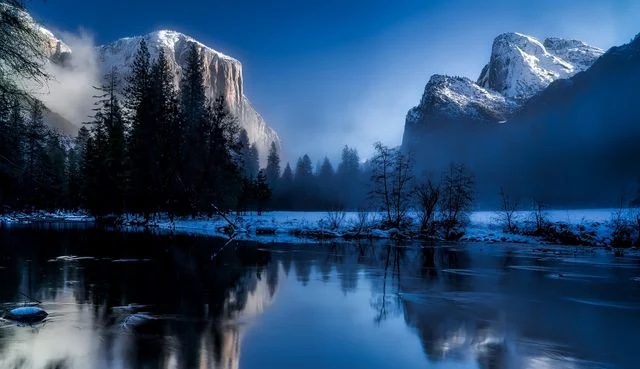
\includegraphics[width=0.5\columnwidth]{figures/View.jpg}
	\vskip 6pt
	\caption{Tek satır olması durumunda ortalı olur. }
	\label{fig:ornek2}
\end{figure}

Şekil~\ref{fig:ornek2}’de gösterildiği gibi \lipsum[1][1].

\section{Tam Sayfa Şekil}
\label{sec:sekil_tam}
Tam sayfa şekil Şekil~ref{fig:landscape}'de verildiği gibi üretilir.
\begin{sidewaysfigure}[htbp] % Rotates the figure horizontally
	\centering
	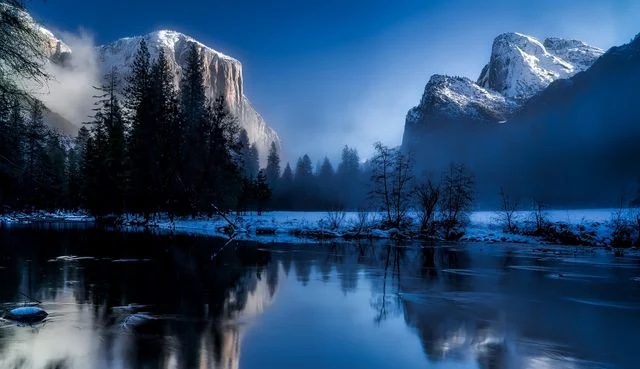
\includegraphics[width=\textheight, keepaspectratio]{figures/View.jpg}
	\caption{Tam sayfa şekil örneği.}
	\label{fig:landscape}
\end{sidewaysfigure}

\lipsum[1 -3]

\section{Çizelge Atıfları ve Çizelge Örneği}
\label{sec:ciz_atif}
Çizelge numarası ve üst yazısı, bir satır aralığı kullanılarak ve yazıdan önce 12 punto, sonra 6 punto aralık bırakılarak yazılmalı ve çizelge üst yazısı nokta ile bitirilmelidir.

Çizelge üst yazısı ile çizelgenin tamamı aynı sayfa içinde yer almalıdır. 

Çizelgeden sonra gelen metin bölümündeki ilk paragraf üstten 12 alttan 6 punto aralık bırakılarak yazılmalıdır. Çizelgelerden hemen sonra gelecek başlıklar, belirtilen başlık formatlarında değişiklik yapılmadan aynen kullanılmalıdır.

Çizelgelerde dipnot kullanılması gerekiyorsa 1 satır aralıklı ve metinden 2 yazı boyutu küçük yazılmalıdır.

Çizelge~\ref{tab:ornek2}'de tek satırlı çizelge yazısı gösterilmiştir. Çok satırlı örnek daha önce sağlanmıştır.
\begin{table}[h]
	\centering
	\caption{Tek satırlı ve kolonlar ortalanmış çizelge.}
	\begin{tabular}{cccc}
		\hline
		Kolon A & Kolon B & Kolon C & Kolon D \\
		\hline
		Satır A & Satır A & Satır A & Satır A \\
		Satır B & Satır B & Satır B & Satır B \\
		Satır C & Satır C & Satır C & Satır C \\
		\hline
	\end{tabular}
	\label{tab:ornek2}
\end{table}
\lipsum[1-3]

\begingroup
\begin{table}[thbp]
	\caption[Birden çok sayfaya dağılan tablo örneği]{Birden çok sayfaya dağılan çizelgenin çok satırlı başlık içeren örneği}
	\label{ciz:multiPageSample}
	\vskip -14pt
\end{table}
\begin{center}
	\addtocounter{table}{-1}
	\begin{longtable}{ll}\hline
		\textbf{Başlık 1}& \textbf{Başlık 2}\\\hline
		\endfirsthead
		\multicolumn{2}{m{1\textwidth}}{%
			\textbf{Çizelge \ref{ciz:multiPageSample} (devam) :} \hspace{0.5em} 
			\parbox[t]{0.65\textwidth}{%
				Bu uzun başlık burada düzgün şekilde hizalanmalı ve birkaç satıra yayılmalıdır.
			}
		} \\ \hline
		\textbf{Başlık 1}& \textbf{Başlık 2}\\ \hline
		\endhead
		\endfoot
		\endlastfoot
		blah blah blah & blah blah blah \\
		& blah blah blah \\
		& blah blah blah \\
		& blah blah blah \\
		& blah blah blah \\
		& blah blah blah \\
		& blah blah blah \\
		& blah blah blah \\
		& blah blah blah \\
		& blah blah blah \\
		& blah blah blah \\
		& blah blah blah \\
		
		blah blah blah & blah blah blah \\
		& blah blah blah \\
		& blah blah blah \\
		& blah blah blah \\
		& blah blah blah \\
		& blah blah blah \\
		
		blah blah blah & blah blah blah \\ \hline
		& blah blah blah \\
		blah blah blah & blah blah blah \\
		& blah blah blah \\
		& blah blah blah \\
		& blah blah blah \\
		& blah blah blah \\
		& blah blah blah \\
		& blah blah blah \\
		& blah blah blah \\
		& blah blah blah \\
		& blah blah blah \\
		& blah blah blah \\
		& blah blah blah \\
		& blah blah blah \\
		& blah blah blah \\
		& blah blah blah \\
		
		blah blah blah & blah blah blah \\
		& blah blah blah \\
		& blah blah blah \\
		
		blah blah blah & blah blah blah \\
		& blah blah blah \\
		& blah blah blah \\
		& blah blah blah \\
		
		blah blah blah & blah blah blah \\
		& blah blah blah \\
		& blah blah blah \\
		& blah blah blah \\
		& blah blah blah \\
		blah blah blah & blah blah blah \\
		& blah blah blah \\
		& blah blah blah \\
		
		blah blah blah & blah blah blah \\
		& blah blah blah \\
		& blah blah blah \\
		& blah blah blah \\
		
		blah blah blah & blah blah blah \\ \hline
		& blah blah blah \\
		& blah blah blah \\
		& blah blah blah \\
		& blah blah blah \\\hline
	\end{longtable}
\vskip -48pt% Boşluk duruma göre bu kısımdan ayarlanabilir.
\end{center}
Çizelge~\ref{ciz:multiPageSample}'de birden çok sayfaya yayılan çizelge örneği normal sayfa düzeni içinde verilmiştir.

\lipsum[1-2]

\begin{landscape} % Entire page in landscape
\begin{table}[thbp]
	\caption[Birden çok sayfaya dağılan yatay tablo örneği]{Birden çok sayfaya dağılan çizelgenin çok satırlı başlık içeren yatay sayfa düzeni örneği}
	\label{ciz:multiPageSample2}
	\vskip -12pt
\end{table}
\begin{center}
	\addtocounter{table}{-1}
	\begin{longtable}{ll}\hline
		\textbf{Başlık 1}& \textbf{Başlık 2}\\\hline
		\endfirsthead
		\multicolumn{2}{m{1\textwidth}}{%
			\textbf{Çizelge \ref{ciz:multiPageSample2} (devam) :} \hspace{0.5em} 
			\parbox[t]{0.85\textheight}{%
			Birden çok sayfaya dağılan çizelgenin çok satırlı başlık içeren yatay sayfa düzeni örneği
			}
		} \\ \hline
		\textbf{Başlık 1}& \textbf{Başlık 2}\\ \hline
		\endhead
		\endfoot
		\endlastfoot
	
		blah blah blah & blah blah blah \\
		& blah blah blah \\
		& blah blah blah \\
		& blah blah blah \\
		& blah blah blah \\
		& blah blah blah \\
		& blah blah blah \\
		& blah blah blah \\
		& blah blah blah \\
		& blah blah blah \\
		& blah blah blah \\
		& blah blah blah \\
		
		blah blah blah & blah blah blah \\
		& blah blah blah \\
		& blah blah blah \\
		& blah blah blah \\
		& blah blah blah \\
		blah blah blah & blah blah blah \\		
		blah blah blah & blah blah blah \vspace{2pt}  \\\hline 
		
		blah blah blah& blah blah blah  \\
		blah blah blah & blah blah blah \\
		& blah blah blah \\
		& blah blah blah \\
		& blah blah blah \\
		& blah blah blah \\
		& blah blah blah \\
		& blah blah blah \\
		& blah blah blah \\
		& blah blah blah \\
		& blah blah blah \\
		& blah blah blah \\
		& blah blah blah \\
		& blah blah blah \\
		& blah blah blah \\
		& blah blah blah \\
		
		blah blah blah & blah blah blah \\
		& blah blah blah \\
		& blah blah blah \\
		
		blah blah blah & blah blah blah \\\hline
		& blah blah blah \\
		& blah blah blah \\
		& blah blah blah \\
		
		blah blah blah & blah blah blah \\
		& blah blah blah \\
		& blah blah blah \\
		& blah blah blah \\
		& blah blah blah \\
		blah blah blah & blah blah blah \\
		& blah blah blah \\
		& blah blah blah \\
		
		blah blah blah & blah blah blah \\
		& blah blah blah \\
		& blah blah blah \\
		& blah blah blah \\
		& blah blah blah \\
		& blah blah blah \\\hline 
	\end{longtable}
\end{center}
\end{landscape}
Çizelge~\ref{ciz:multiPageSample2}'de birden çok sayfaya yayılan çizelge örneği yatay sayfa düzeni içinde verilmiştir. \lipsum[1][1-6]

\chapter{METİNLER}
\label{chap:metin}
\section{Gövde Metinleri}
\label{sec:govde}
\lipsum[1][1-6]

\subsection{Sayfa marjinleri-Sayfa boşlukları}
\label{sub:sayfa}
Sayfa altı boşluğu 2.5 cm’dir. Bundan daha fazla gereksiz boşluk kalması yanlıştır (Yani bu boşluğun olmaması gerekir). Sayfalardaki metin, çizelge, şekil, vs. bu gözetilerek dengelenmelidir.
\begin{itemize}
	\item Şekiller, çizelgeler büyütülebilir, küçültülebilir.
	\item Şekil ve çizelgeler ait açıklama metinleri (ilk atıf olandan hariç) duruma göre
	şekil ve çizelge öncesine veya sonrasına konulabilir.
	\item Şekil ve çizelgeler uygun en yakın yere konulur. Bu uygunluk sayfa altı boşluklar düşünülerek karar verilmelidir.
\end{itemize}
Benzeri çözümlerle zorunlu durumlar hariç sayfa altı ve üstü boşluklar bırakılmaz.

\subsection{Denklemler}
\label{sub:denklem}
Denklemlere öncesinde atıfta bulunmaktan kaçınılmalıdır. Parametreler denklemin altında tek tek açıklanmalıdır.
\beq
\label{denk1}
{\mathbf y}={\mathbf H}{\bf \Psi}{\mathbf x} + {\bm{\nu}}. 
\eeq
denklemde $y$ çıkış vektörünü, $x$ giriş vektörünü $H$ ve $\Psi$ ilgili matrisleri $\nu$ Gauss gürültüyü ifade etmektedir.
Denklem~\ref{denk1} birçok alanda kullanılmaktadır.

Çok satırlı denklemlerde benzer strateji takip edilerek oluşturulabilir. Bir önceki bölümde belirtilen sinyal modeli kullanılarak, ${\mathbf z}$ $0$ ortalamalı Gauss vektör oluşturur, bu durumda ${\bf m}_{\bf z}$, aşağıdaki gibi hesaplanabilir 
\bea{\bf m}_{\bf z} &=& \mbox{E} \left[{\bf z}\right]= \sqrt{\frac{\rho K}{K+1}}\left( \bar{\bf h}_u \psi_u X_v -\bar{\bf h}_{\hat{u}} \psi_{\hat{u}} X_{\hat{v}}\right)\nnl
&=&\sqrt{\frac{\rho K}{K+1}}\left( \bar{\bf h}_u a_u X_v e^{j\theta_u}-\bar{\bf h}_{\hat{u}} a_{\hat{u}} X_{\hat{v}}e^{j\theta_{\hat{u}}}\right)\eea ve kovaryans matrisi,  ${\bf \Sigma}_{\bf z}$, aşağıdaki gibi bulunur:
\beq
{\bf \Sigma}_{\bf z} =\frac{\rho  \gamma(u, \hat{u}, v, \hat{v}, \psi_u, \psi_{\hat{u}}) {\bf \Sigma}_r}{K+1}
\eeq 

Buna ek olarak birden fazla denklem de aşağıda gösterildiği gibi peş peşe sıralanabilir. Bu denklemler ileride tek tek alıntılanacaksa hepsinin label komutu ile ayrı ayrı etiketlenmesi gerekmektedir. Ayrıca manuel alıntılama da kullanılabilir. Ancak bu durumda yeni denklem eklenmesi durumunda numaraların değişebileceği göz önünde bulundurulmalıdır.
\bea
\label{denklem2}
\Gamma^{(n)}_{\hat{U}_1} &=& \frac{P_n |h_n|^2}{P_{N+n} |h_{N+n}|^2 + \sigma^2} = \frac{P_t |g_n|^2}{\epsilon P_t |g_{N+n}|^2 + \sigma^2} \\
\label{denklem3}
\Gamma^{(n)}_{U_2} &=& \frac{P_{N+n} |h_{N+n}|^2}{P_n |a_n - \hat{a}_n|^2 |h_n|^2 + \sigma^2} \nonumber \\
&=& \frac{\epsilon P_t |g_{N+n}|^2}{P_t |a_n - \hat{a}_n|^2 |g_{n}|^2 + \sigma^2}\\
\label{denklem4}
\Gamma^{(k)}_{\tilde{U}_1} &=& \frac{P_{k} |h_{k}|^2}{\sigma^2} = \frac{P_t |g_{k}|^2}{\sigma^2}
\eea
Çoklu denklem alıntılama Denklemler~\ref{denklem2},~\ref{denklem3} ve \ref{denklem4} şeklinde yapılabilir.

\chapter{ATIFLAR, ALINTILAR VE DİPNOTLAR}
\label{chap:atif}
Bu bölümde atıflar, alıntılar ve dipnotların nasıl olması gerektiği hakkında kısaca bilgi
verilecektir.
\section{Atıflar (Kaynakların Metin İçinde Gösterimi)}
\label{sec:atif}
Atıfların metin içinde gösteriminde IEEE olarak bilinen köşeli parantez içinde atıf verme yöntemi önerilir. Yazar soyadı ile atıf vermek ve kaynakça oluşturmak daha manuel bir süreç olduğu için önerilmez. Her iki durumda da atıfların nasıl verileceği aşağıdaki bölümlerde açıklanmıştır.
\subsection{Yazar soyadına göre atıf verme}
\label{sec:soyad}
Kaynaklar metin içinde yazar soyadı ve tarih belirtilerek verilir. Kaynaklar sayfasında yazar soyadına göre alfabetik olarak sıralama yapılır. 

Metin içinde kaynak, cümlenin başlangıcında veya içinde verilecekse, Bayhan (2015)
şeklinde, kaynak cümle sonunda verilecekse (Bayhan, 2015). şeklinde gösterilir.
Nokta işareti kaynaktan hemen sonra konur.

Kaynak birden fazla yazara ait olduğunda, yazar sayısı iki ise, cümle başında veya
içinde Ertaş ve Bayhan (2017) şeklinde, cümle sonunda ise (Ertaş ve Bayhan, 2017).
şeklinde yazılır.
Yazar sayısı ikiden fazla ise cümle başında veya içinde Bayhan ve diğ. (2018) şeklinde, cümle sonunda ise (Bayhan ve diğ, 2018). şeklinde yazılır.

Aynı yazara ait ve aynı yıl içinde yayınlanmış yayınlar Saray (2015a), Saray (2015b) şeklinde numaralandırılır.

Aynı parantez içerisinde aynı yazarın 2 ve daha fazla eserine atıfta bulunma; son yayınlanan eseri en son belirterek aynı parantez içerisinde gösterilebilirler. Örneğin;
Past research (Can, 1990, 2006, baskıda).

Eserin belirli bir bölümüne atıfta bulunma; bir eserin sadece bir bölümüne, sayfasına, çizelgeye, şekle ya da eşitliğe atıfta bulunurken daima sayfa numarası gösterilmelidir. Sayfa ifadesinin kısaltılmış biçimi kullanılırken bir bölüme atıfta bulunurken “bölüm”
ifadesinde kısaltmaya gidilmez. Örneğin; (Afet Koordinasyon Merkezi, 2015, s. 15),
(Barka, 1999, Bölüm 5).

Aynı parantez içerisinde 2 ya da daha fazla esere atıf; (Akcan, 2017; Can, 2016).

Metinde kişisel görüşmeye atıfta bulunma; (A. E. Akay, kişisel görüşme, 7 Şubat
2017), (O. T. Can, kişisel görüşme, 8 Şubat 2017).

İkincil kaynak (atıf yapılan kaynak başka bir kaynağa atıfta bulunuyorsa) metinde
orijinal kaynağa atıfta bulunulur ve parantez içerisinde orijinal kaynağa atıfta bulunan
yazara gönderme yapılır. Referans listesinde sadece orjinal kaynağa atıfta bulunan
kaynak için giriş yapılır; orijinal kaynak için referans girişi yapılmaz. Örnek: Bayhan,
Marmara Bölgesinin güneyinin de İstanbul kadar deprem tehlikesi altında olduğunu
öne sürmektedir (Özdemir, 2016’da atıfta bulunulduğu gibi).

\subsection{Numara ile atıf verme}
\label{sec:soyad}
Metin içinde [ ] köşeli parantez içinde numaralandırılır. Tezde ilk verilen kaynak [1]
numara ile başlar ve veriliş sırasına göre numaralandırılır. Bunun için özel bir organizasyon yapılmasına gerek yoktur. Bu yöntemde atıf vermenin en kolay yolu latex için .bib uzantılı bir bibliyografya dosyası oluşturarak cite komutu ile buradaki kaynaklara atıf vermektir.

Tek bir kaynağa atıf verilen bir cümle örneği şudur\cite{ArticleRef}. Eğer birden fazla kaynağa atıf verilecekse yazım şu hale dönüşür\cite{ArticleRef,BookRef}. İkiden fazla peş peşe gelen kaynaklara atıf verilecekse latex otomatik olarak ilk ve son kaynak nosunu vererek araya kısa çizgi atar \cite{ArticleRef,BookRef,ConferenceRef}. Peş peşe ve ayrı örnekler bir arada ise uygun yöntemi latex derleyicisi kendisi belirleyecektir, ayrıca numaralandırmayı da otomatik olarak yapacaktır \cite{ArticleRef,BookRef,ConferenceRef,ManualRef}.
\section{Alıntılar}
\label{sec:alinti}
Genel olarak alıntılar kelime, imla ve noktalama bakımından aslına uygun olarak yapılır. Alıntı yapılan parçada bir yanlış varsa, doğrusu köşeli parantez içerisinde belirtilmek koşuluyla metin aynen nakledilir.

Kırk kelimeden daha az uzunluktaki kısa alıntılar çift tırnak içerisinde verilir. Alıntının sonunda ilgili kaynağa atıf yapılıp atıftan sonra nokta koyulur. Aydan vd.’e göre (1998), "Alıntı alıntı alıntı alıntı alıntı alıntı alıntı alıntı" (s. 20).

Kırk kelimeden fazla olan uzun alıntılar tırnak içerisinde gösterilmezler. Uzun alıntılar soldan 1 sekme  içerden verilir. İçerden verilen uzun alıntılarda, 2 yazı karakteri daha küçük karakter kullanılır. Ancak, çok sık ve çok uzun alıntılardan kaçınılması tavsiye edilir. Kısa alıntılardan farklı olarak noktalama atıftan sonra değil de önce yapılır. Örneğin; .(s. 196) gibi.
\begin{quote}
	\lipsum[1-2]
	Alıntı burada bitmektedir. (Bayhan, 2017, ss. 88-89)
\end{quote}

Alıntılar için daha detaylı bilgi edinmek için yazım kılavuzuna bakınız.
\section{Dipnotlar}
\label{sec:dip}
Tezlerde içeriği genişletici, güçlendirici veya ilave nitelikteki bilgiler (içerik dipnotu) kullanılabilir\footnote{Dipnotlar ile kaynak gösterimi yapılmaz. Dipnotlar tez içerisinde içeriği genişletici, güçlendirci veya ilave nitelikteki bilgileri vermek için kullanılır. Verilen genişletici, güçlendirci veya ilave nitelikteki bilgiler zorunlulukla kaynak içeriyorsa bu kaynak mutlaka kaynaklar bölümünde verilmelidir.}.

Dipnot numaraları metnin hemen sonuna koyulur. Metin paragrafsa dipnot numarası paragrafın son kelimesinin üzerine, bir kavram veya isimse, bu defa kavram veya ismin hemen üzerine yazılır.

Metin içerisindeki dipnot numarası; satır hizasının üzerinde\footnote{Dipnot, ilgili sayfanın altına metinden 2 karakter küçük yazı ile yazılmalıdır.} şeklinde görünür olmalıdır. Numara sonrasında herhangi bir noktalama işareti konmamalıdır.

Dipnot, bu sayfada gösterildiği gibi metinden 2 karakter küçük yazı ile yazılmalıdır. İlgili metin ile aynı sayfada olmalıdır. 

Dipnot çizgisi ile dipnot numarası arasında bir aralık; dipnot numarası ile dipnotun ilk satırı arasında ise yarım aralık bırakılmalıdır. Dipnotlar metinden ince yatay bir çizgi ile ayrılmalıdır. 

Dipnotlarla ilgili ayrıntılı bilgiler enstitülerin internet sitelerinden ve ilgili bağlantılardan bulunabilir.

\chapter{GEREKLİ İSE BÖLÜM 5}
\label{chap:bolum5}
\lipsum[1][1-6]
\section{Çalışmanın Uygulama Alanı 1}
\label{sec:bolum51}
\lipsum[1][1-5]
\section{Çalışmanın Uygulama Alanı 2}
\label{sec:bolum52}
\lipsum[1][1-5]
\subsection{Çalışmanın uygulama alanının eleştirisi}
\label{subsec:bolum521}
\lipsum[1][1-7]
\subsubsection{Çalışmanın uygulama alanının eleştirisinin eleştirisi}
\label{subsec:bolum5211}
\lipsum[1][1-5]
\paragraph{Beşinci derece başlık}
Beşinci ve daha alt dereceden başlıklar numaralanmaz, içindekiler listesinde yer almaz. \lipsum[1][1-5]

\chapter{SONUÇ VE ÖNERİLER}
\label{chap:bolum6}
\lipsum[1][1-6]
\section{Çalışmanın Uygulama Alanı}
\label{sec:bolum61}
\lipsum[1][1-5]
\section{Sonuçlar ve Öneriler}
\label{sec:bolum62}
\lipsum[1][1-5]
\subsection{Sonuçlar}
\label{subsec:bolum621}
\lipsum[1][1-7]
\subsection{Öneriler}
\label{subsec:bolum622}
\lipsum[1][1-5]

\nocite{*}
\bibliographystyle{styles/tez_v1.bst} %Still may have problems
\bibliography{references} %Referanslar bu bibliyografya dosyasının içindedir.
 
 
 
\chapter*{APA İÇİN KAYNAKLAR}
\singlespacing

\leftskip 25mm \parindent -22mm \textbf{Abrahart, R. J. \& See, L.} (1998). Neural Network vs. ARMA Modelling: Constructing Benchmark Case Studies of River Flow Prediction.In J.Blenc, (Ed.), \textit{GeoComputation ’98. Proceedings of the Third International Conference on GeoComputation}, (pp.145-154). United Kingdom : University of Bristol, September 17-19.

\leftskip 25mm \parindent -22mm \textbf{Abrahart, R. J. \& See, L.} (2000). Comparing neural network and autoregressive moving average techniques for the provision of continuous river flow forecasts in two contrasting catchments, \textit{Hydrological Processes},14 (2), 2157–2172.


\setlength{\parindent}{0pt}  % Remove paragraph indentation
\setlength{\leftskip}{0pt}  % Reset left margin indentation
\setlength{\rightskip}{0pt} % Reset right margin indentation

\appendix
\singlespacing
\chapter{HARİTALAR}
\begin{figure}[htbp]
	\centering
	\subfigure[]{
		
\includegraphics[width=0.45\textwidth]{figures/Comp.jpg}
	}
	\subfigure[]{
		
\includegraphics[width=0.45\textwidth]{figures/Comp.jpg}
	}
	
	\subfigure[]{
		
\includegraphics[width=0.45\textwidth]{figures/Comp.jpg}
	}
	\subfigure[]{
		
\includegraphics[width=0.45\textwidth]{figures/Comp.jpg}
	}
	\caption{2x2 şekil listesi. (a) Bilgisayar 1 (b) Bilgisayar 2 (c) Bilgisayar 3 (d) Bilgisayar 4}
	\label{fig:2x2grid}
\end{figure}

\chapter{ÇİZELGELİ VE YAZI İÇEREN EK}
\lipsum[1-3]
\begin{table}[h]
	\centering
	\caption{Eklerde çizelge örneği}
	\begin{tabular}{cccc}
		\hline
		Kolon A & Kolon B & Kolon C & Kolon D \\
		\hline
		Satır A & Satır A & Satır A & Satır A \\
		Satır B & Satır B & Satır B & Satır B \\
		Satır C & Satır C & Satır C & Satır C \\
		\hline
	\end{tabular}
	\label{tab:ornekapp}
\end{table}
\chapter*{ÖZGEÇMİŞ}
\singlespacing
\begin{table}[h]
	\begin{flushright}  % Align table to the right
		\begin{tabular}{p{0.6\textwidth} p{0.3\textwidth}}  % Two columns
			& 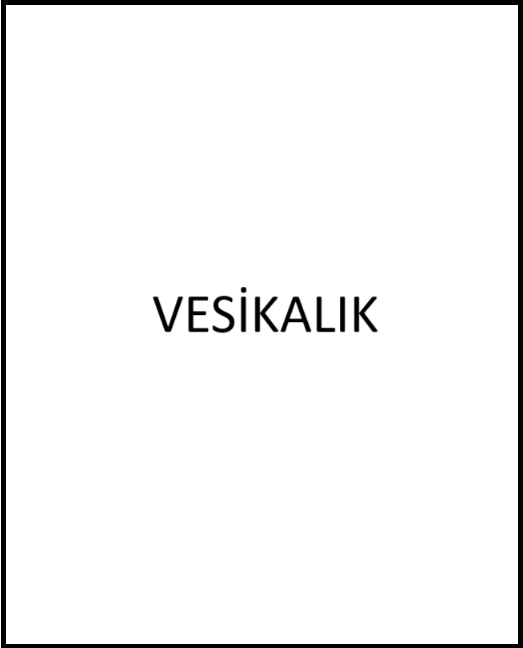
\includegraphics[width=3.5cm]{figures/vesikalık.png} \\  % Fotoğrafınız buraya gelmeli. Şekil olarak eklenmeli.
		\end{tabular}
	\end{flushright}
\end{table}

\begin{table}[h]
	\begin{tabular}{lcr}  % Two columns
			\textbf{Ad-Soyad}&\textbf{:}&  \\  % Fotoğrafınız buraya gelmeli. Şekil olarak eklenmeli.
			\textbf{Doğum Tarihi ve Yeri}&\textbf{:}& \\
			\textbf{E-posta}&\textbf{:}&
	\end{tabular}
\end{table}

\paragraph{ÖĞRENİM DURUMU}

\begin{table}[h]
	\begin{tabular}{lcr}  % Two columns
		\textbf{Lisans}&\textbf{:}&  \\  % Fotoğrafınız buraya gelmeli. Şekil olarak eklenmeli.
		\textbf{Yüksek Lisans}&\textbf{:}& 
	\end{tabular}
\end{table}

\paragraph{MESLEKİ DENEYİM VE ÖDÜLLER:}
\begin{itemize}
	\item Deneyim 1
	\item Deneyim 2
	\item Ödül 1
\end{itemize}

\paragraph{TEZDEN TÜRETİLEN ESERLER, SUNUMLAR VE PATENTLER:}
\begin{itemize}
	\item Yayın 1
	\item Yayın 2
	\item Sunum 1
\end{itemize}

\paragraph{DİĞER ESERLER, SUNUMLAR VE PATENTLER:}
\begin{itemize}
	\item Eser 1
	\item Yayın 1
	\item Patent 1
\end{itemize}






\end{document}